\section{WC 31/3/25}

\subsection*{Overview:}
This week I spent more time working on my artifact
\subsection*{Achievements, Thoughts and Ideas:}
With the majority of my remaining artifact planned out and ready to build these next few weeks are mainly focused on implementation.

Ensuring I keep improving a wide variety of skills I also completed research on: \nameref{research:Plagiarism} in which I learnt about the differences between correctly referring to prior work and unfairly plagiarising from it. I extended the research by focusing on the law regarding use of others code (e.g. using libraries such as Vue JS). To ensure I fully comply with their licensing terms I will need to create an attribution page with links to more resources about each library used.

The rest of my week was spent fixing some bugs that were reported by a couple of friends using my project and developing new features. One Main issue I found was that my dashboard display wasn't scaling quite as I had hoped. My intention was for the content to fit on a single screen span so that the user doesn't have to scroll at all to see all of the information (like how most application dashboards work). Here are some images of the issues faced
\begin{figure}[H]
    \centering
    \begin{minipage}{0.48\textwidth}
        \centering
        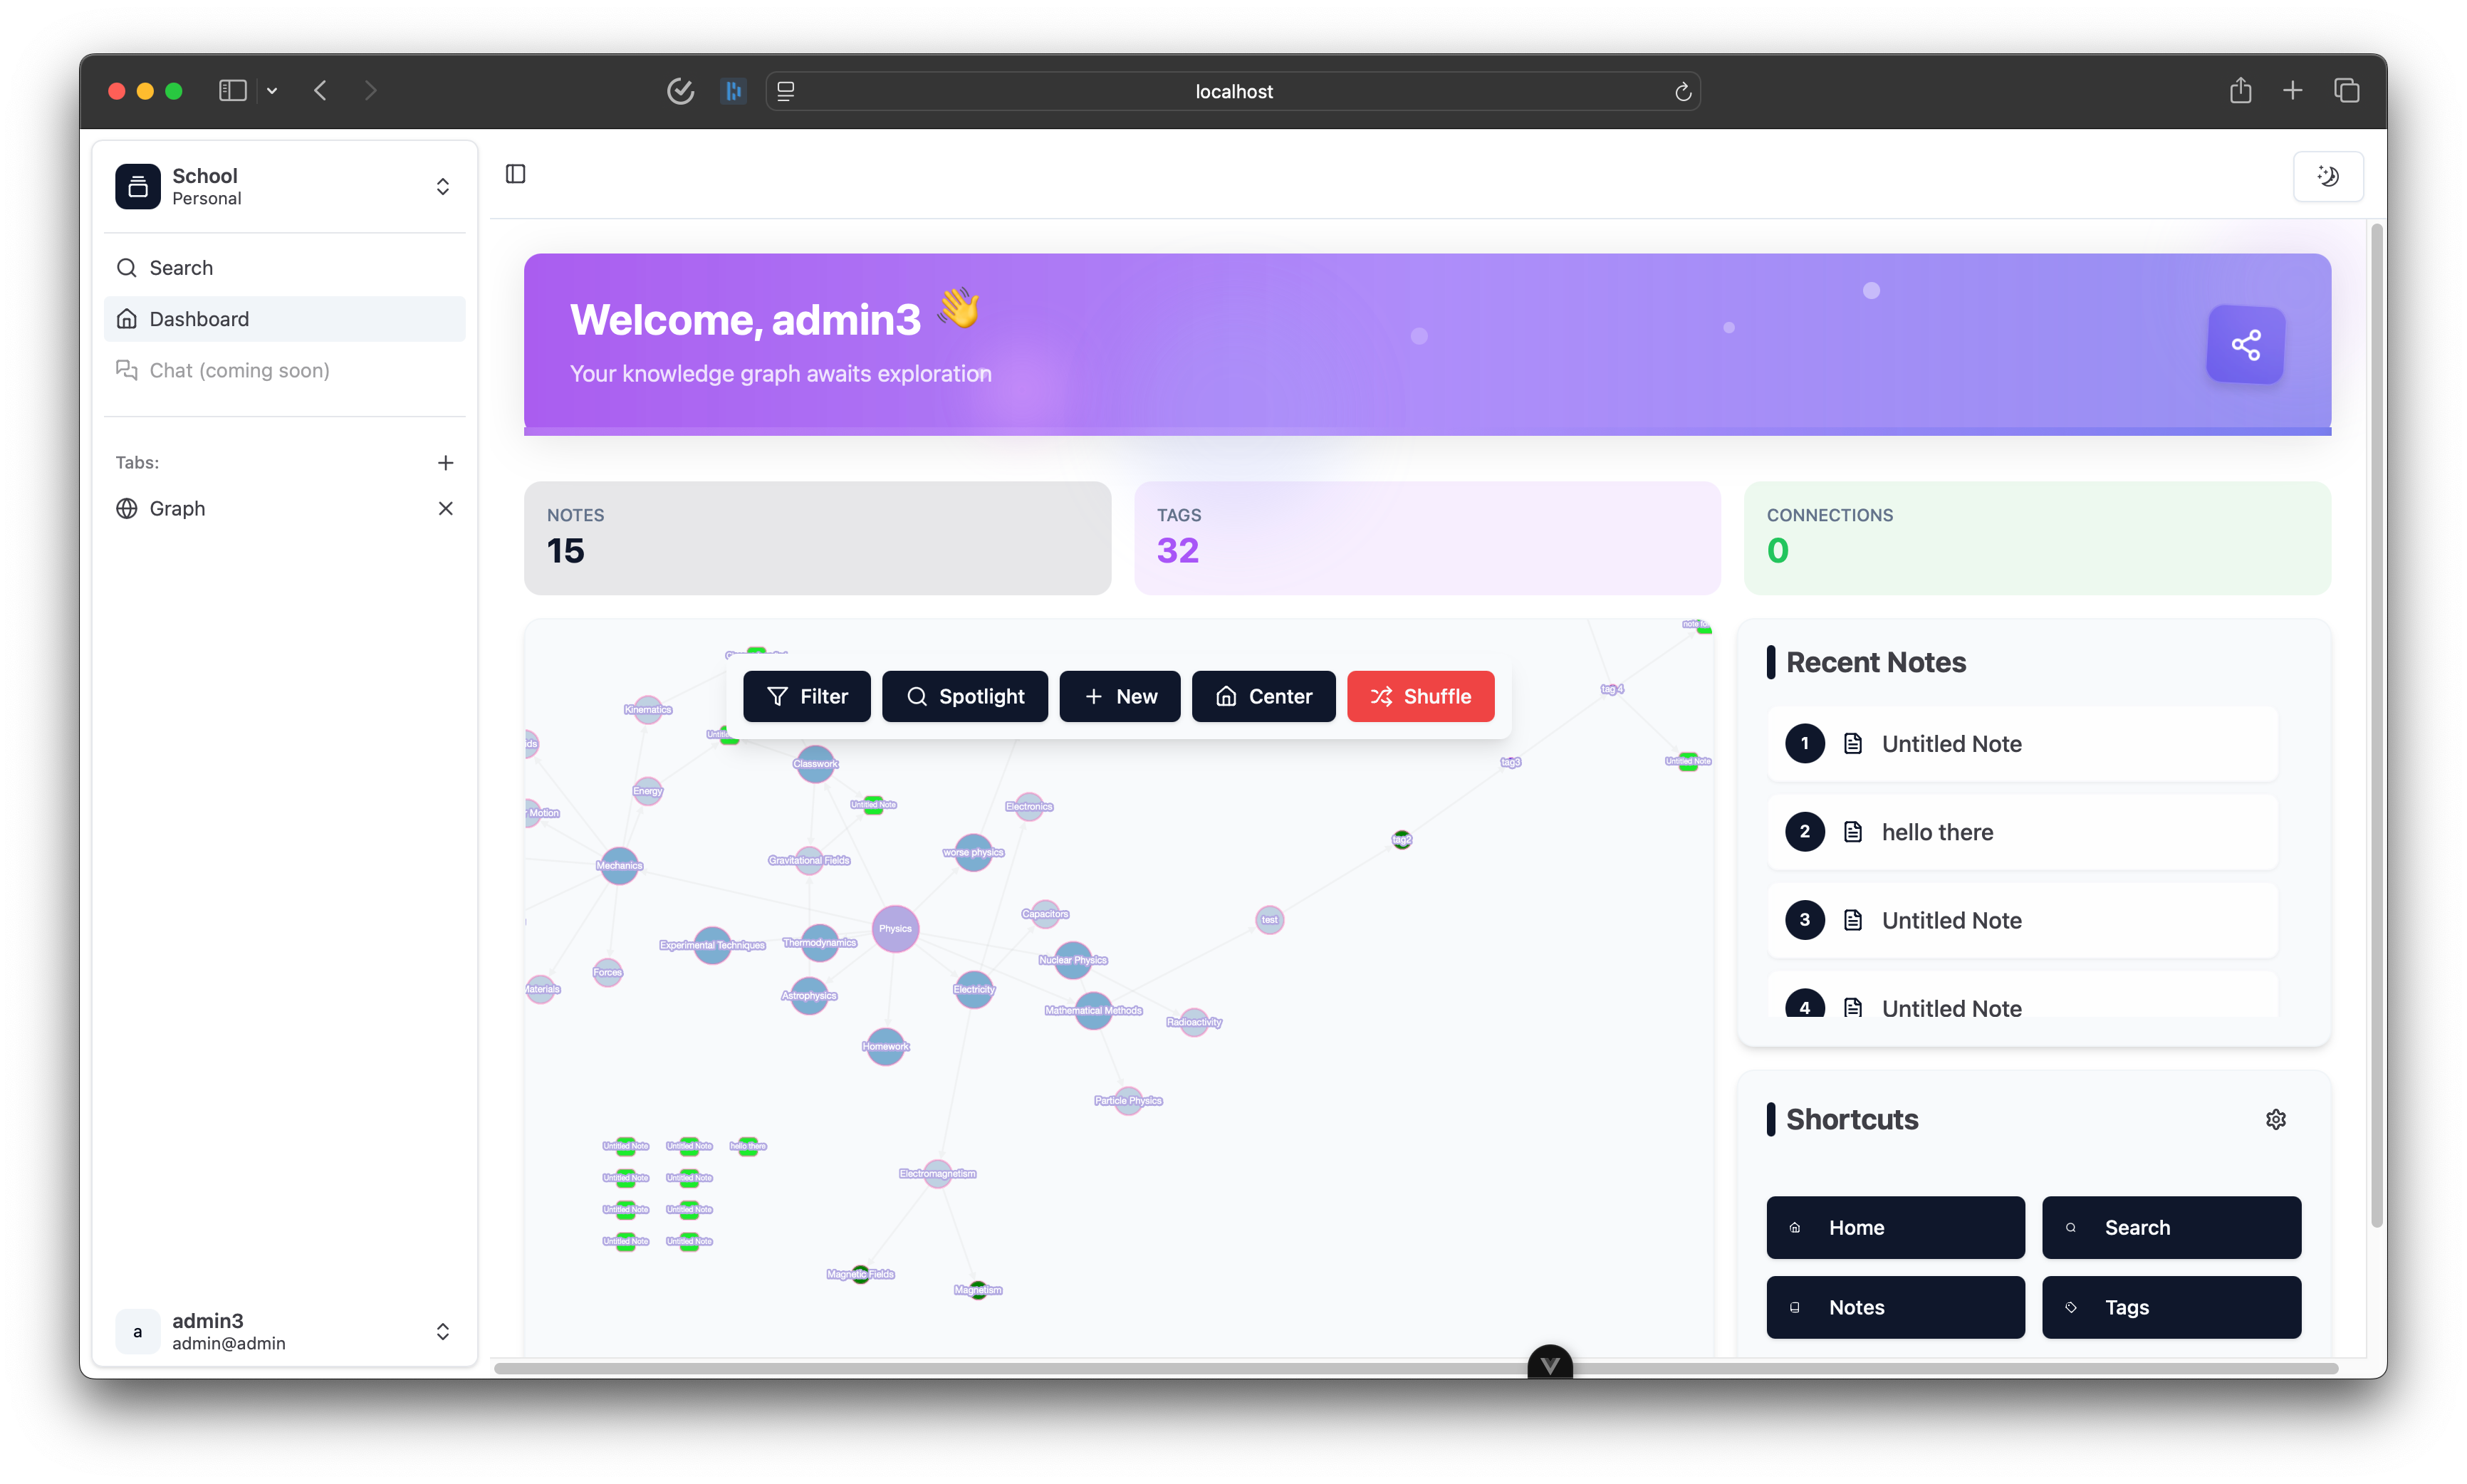
\includegraphics[width=\linewidth]{Diary/24_WC_31-3-25/media/bannerOverflow.png}
        \caption{Overflow as the banner pushes the content down}
        \label{fig:dashboard_issue1}
    \end{minipage}\hfill
    \begin{minipage}{0.48\textwidth}
        \centering
        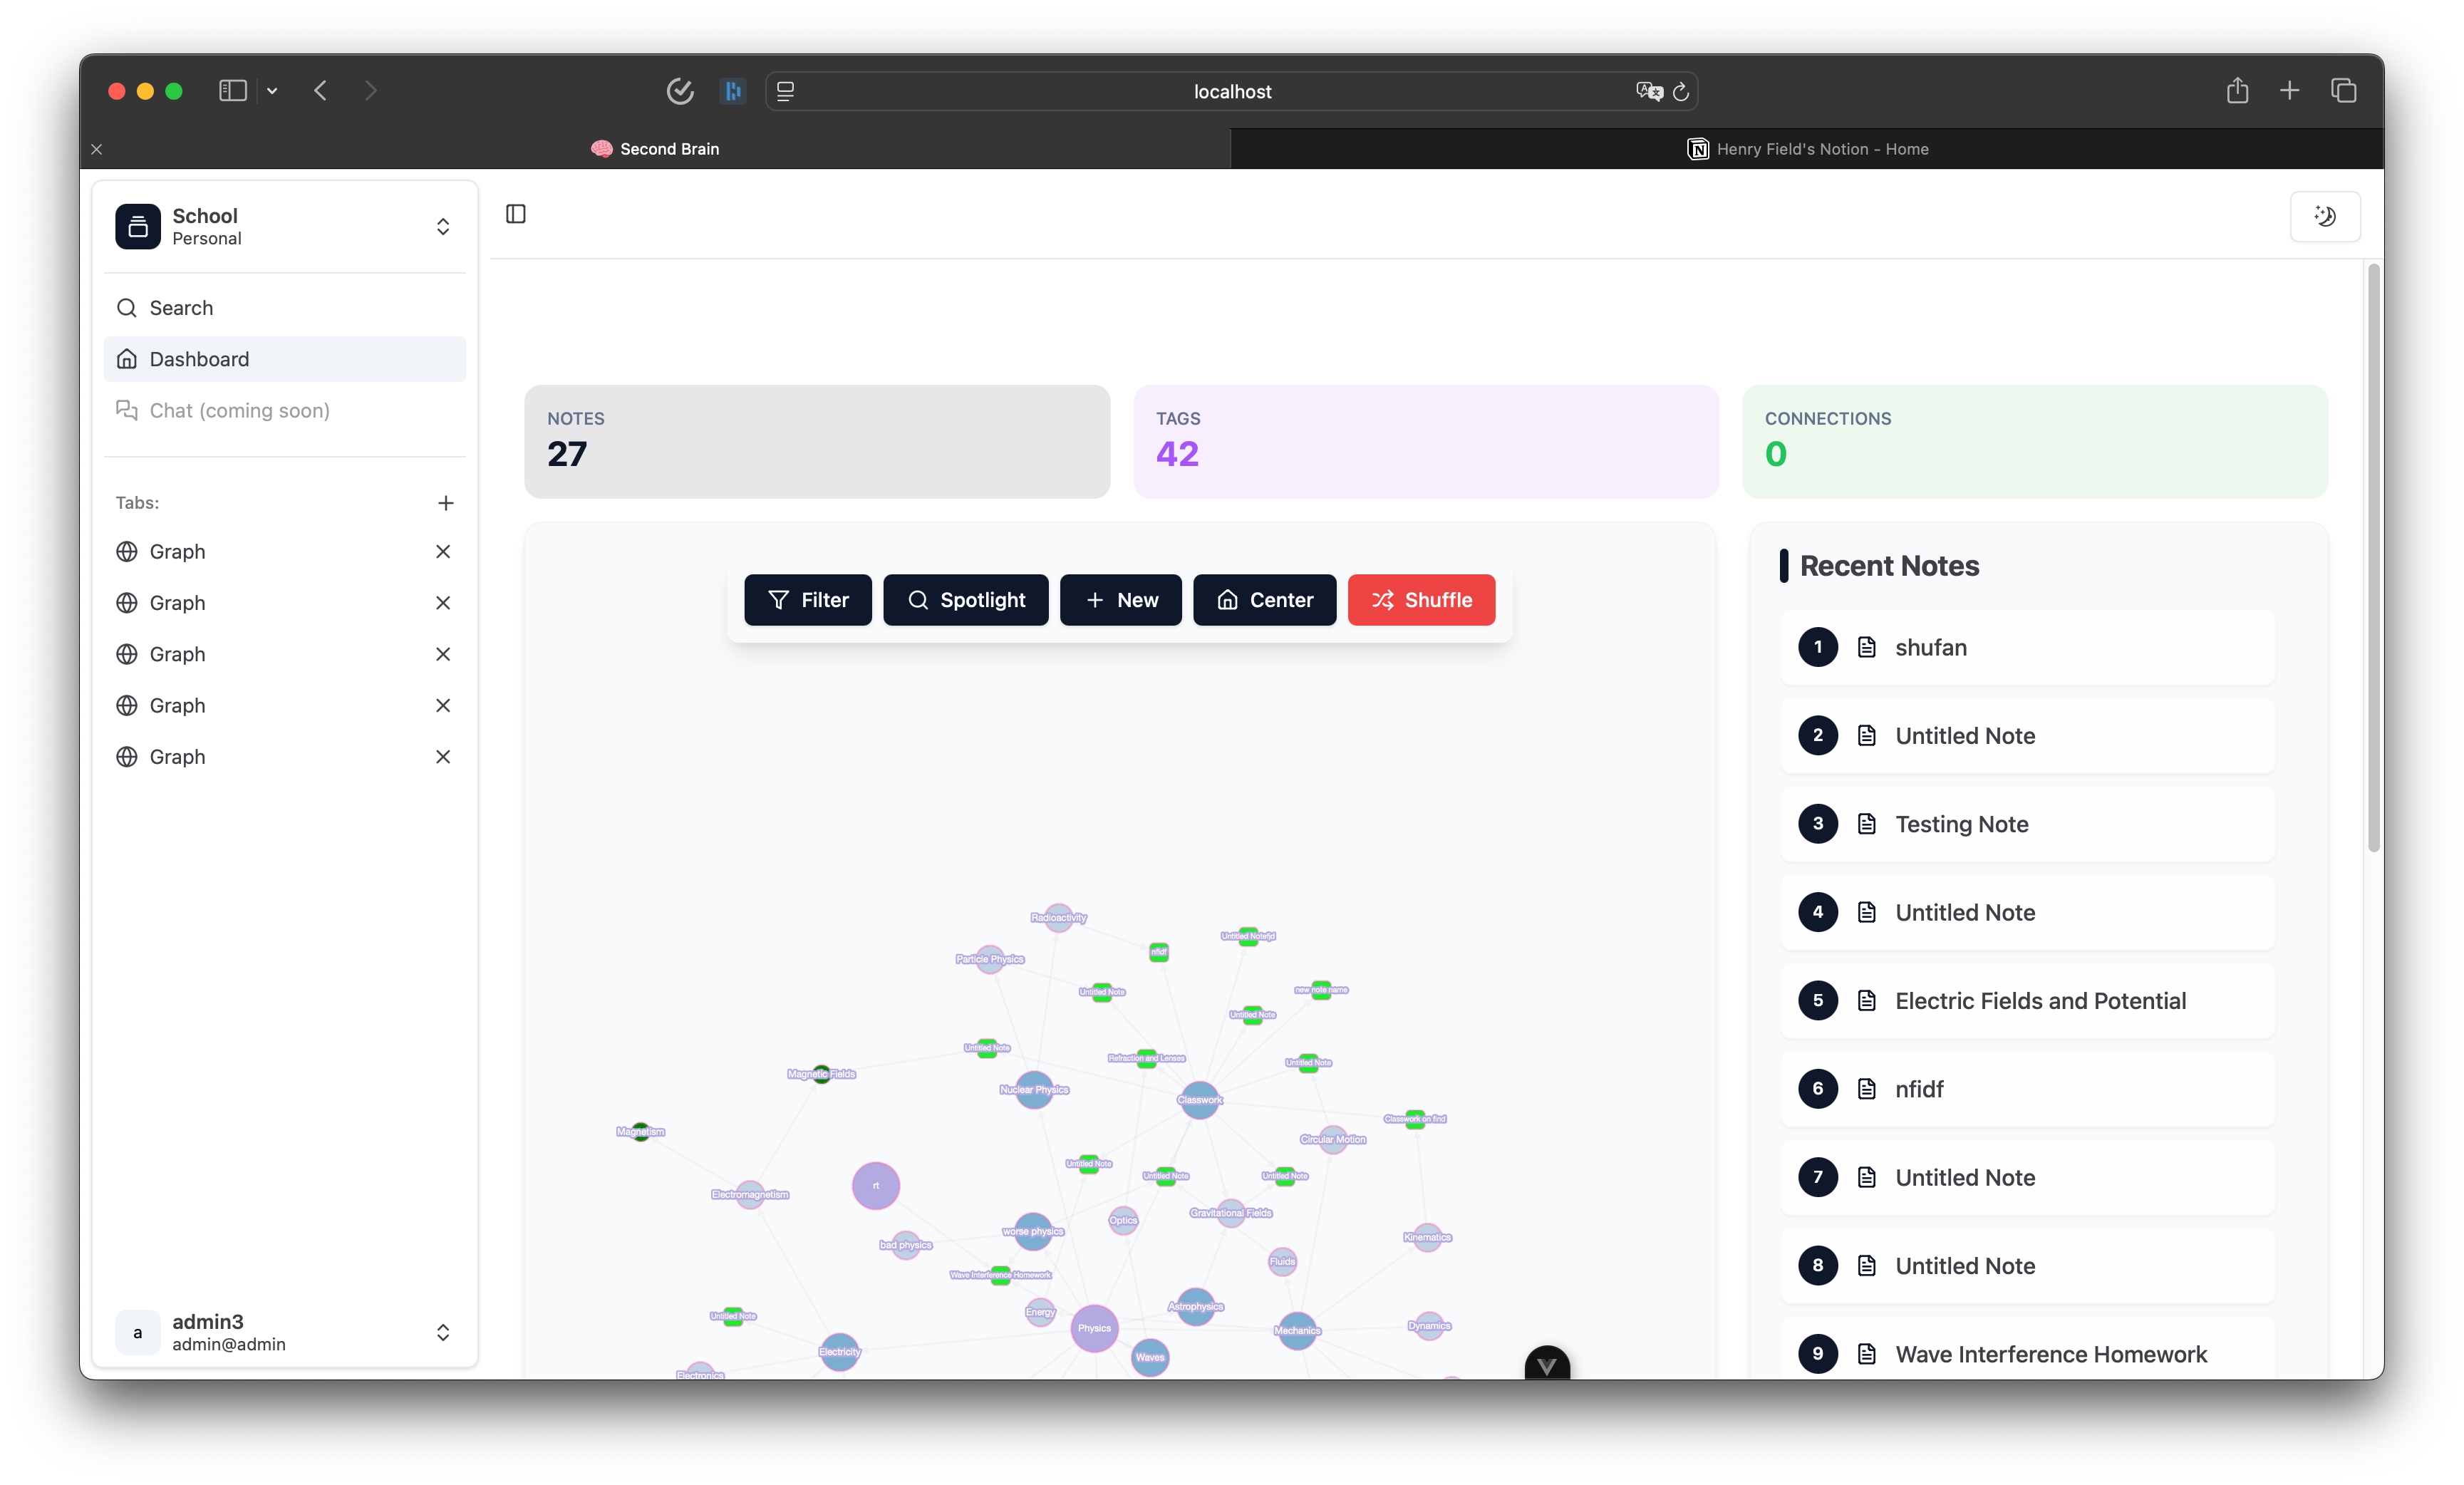
\includegraphics[width=\linewidth]{Diary/24_WC_31-3-25/media/otherOverflow.png}
        \caption{With Banner removed content still overflows}
        \label{fig:dashboard_issue2}
    \end{minipage}
\end{figure}

I initially thought I had solved the issue once I saw a prototype had every box perfectly fitting:
\begin{figure}[H]
    \centering
    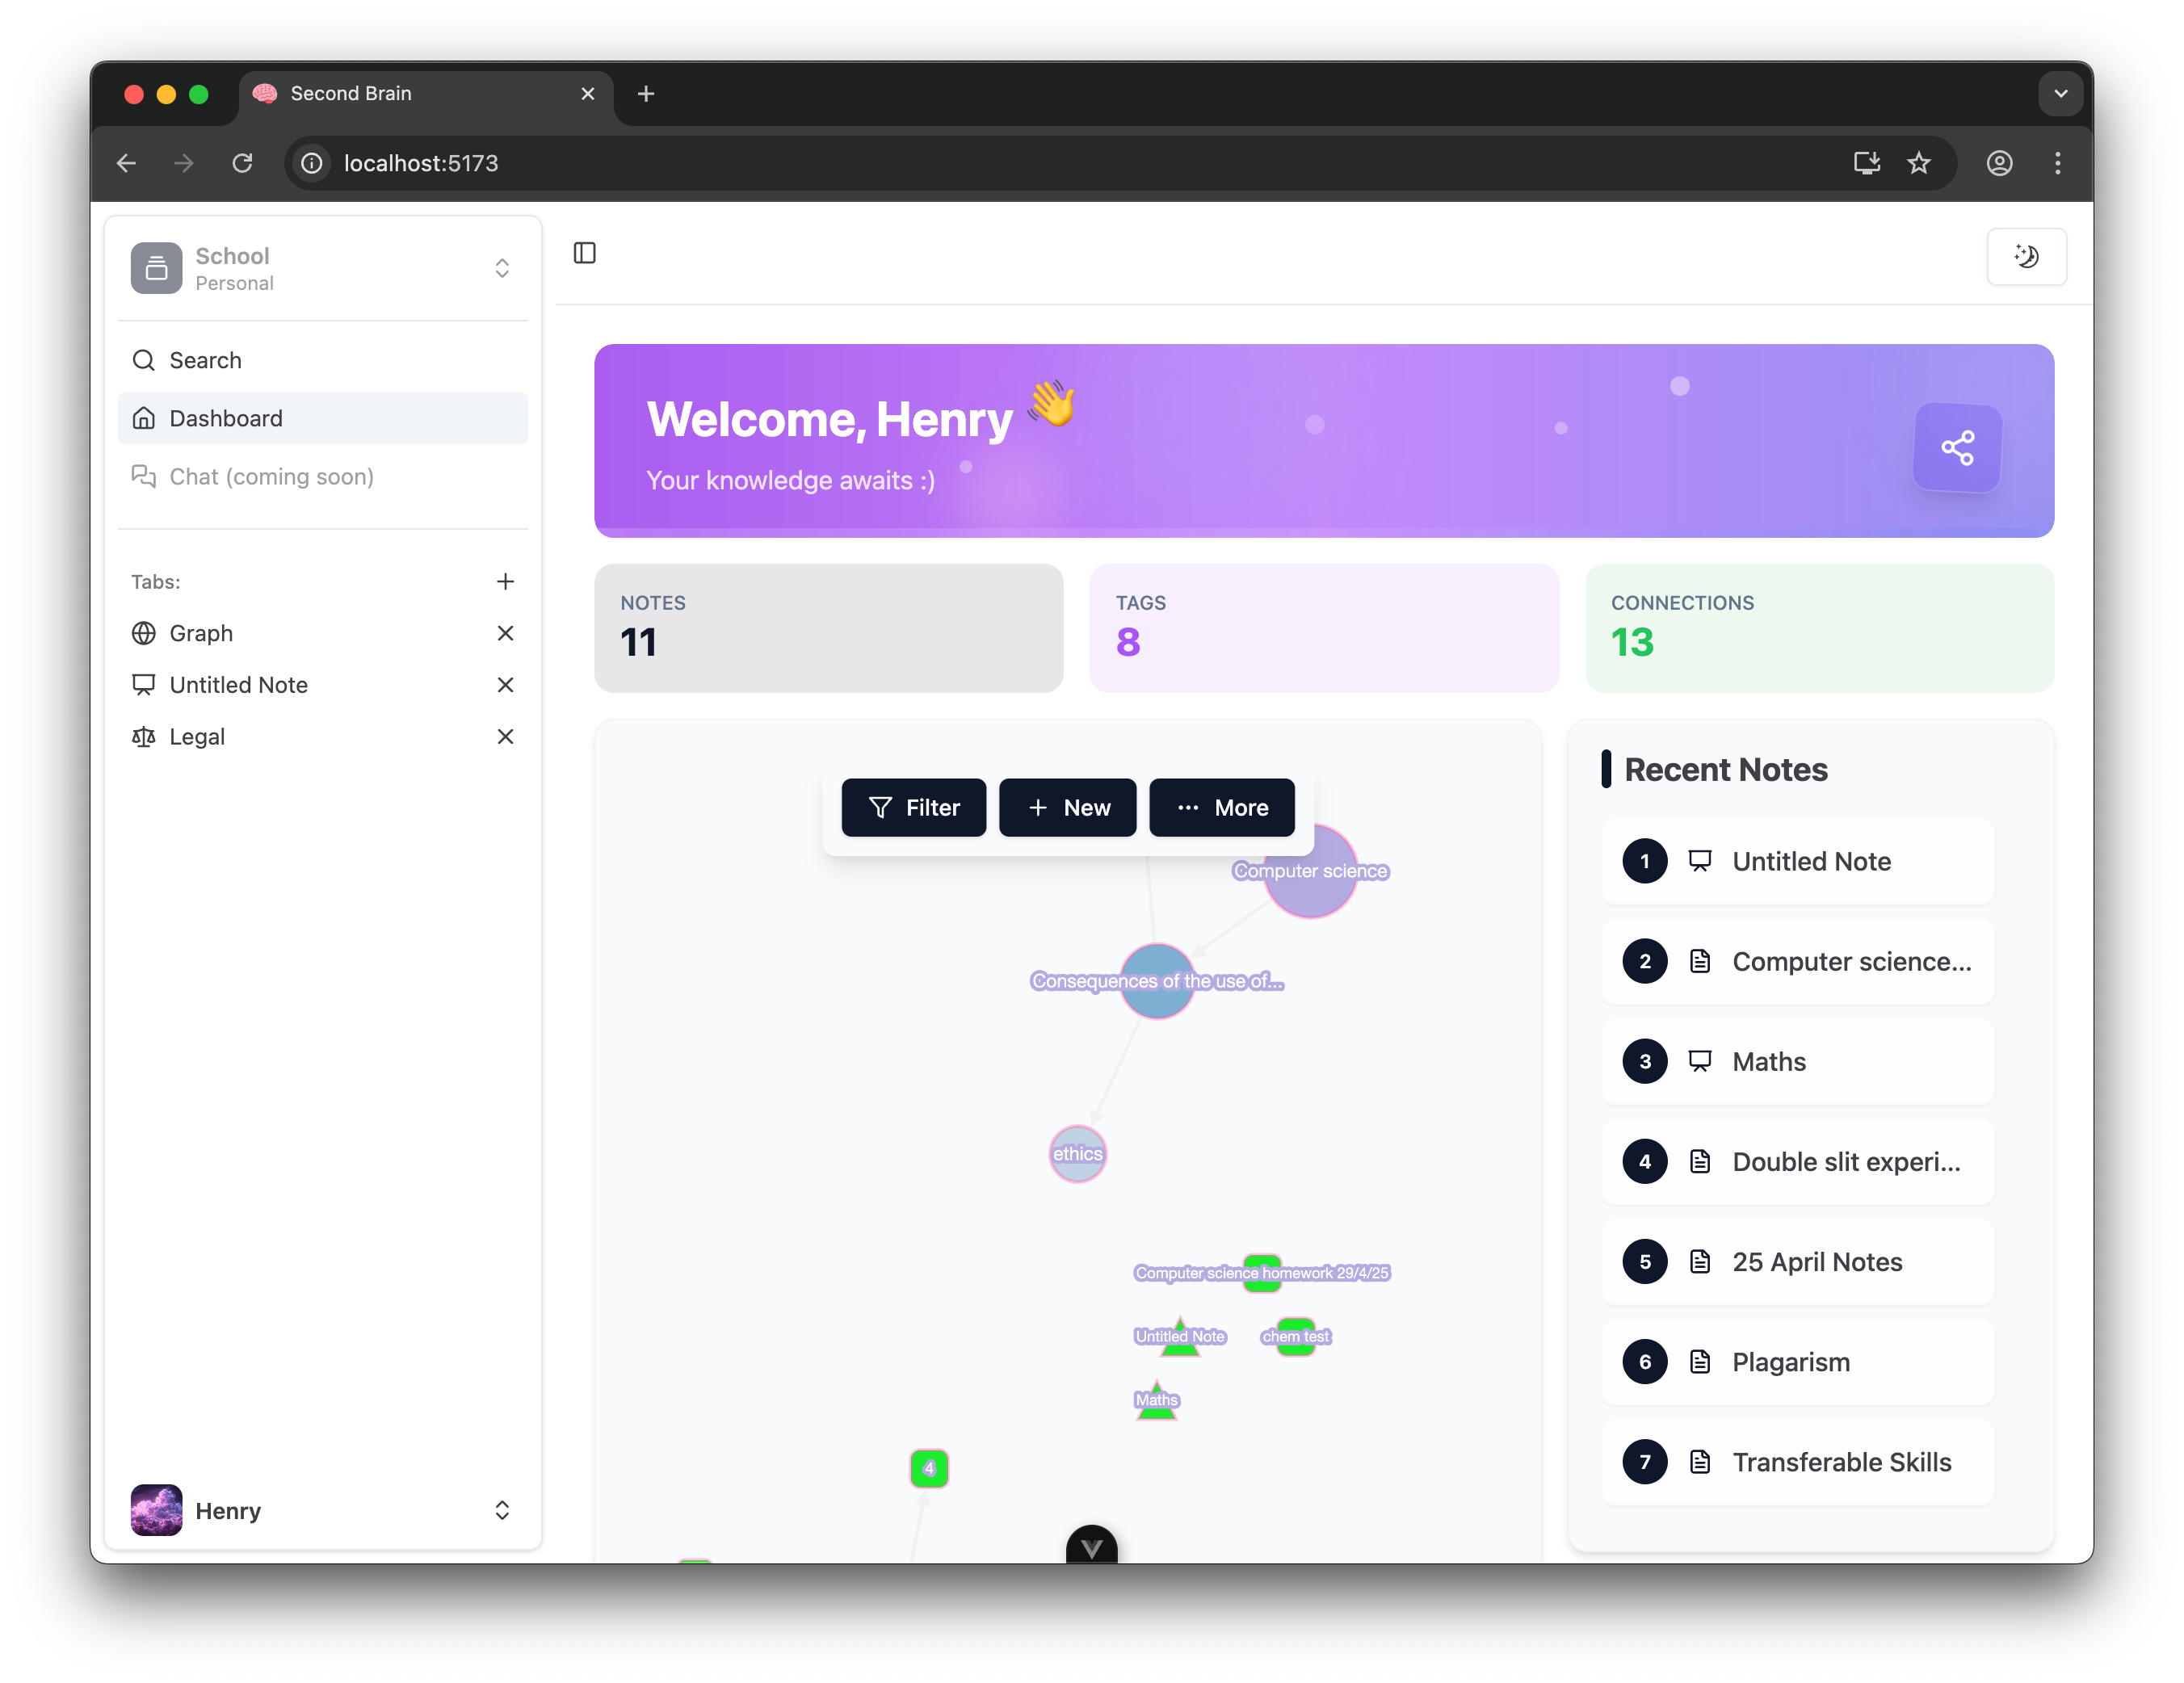
\includegraphics[width=0.8\linewidth]{Diary/24_WC_31-3-25/media/thoughtWasFixed.png}
    \caption{Turns out this was not fixed}
    \label{fig:dashboard_prototype}
\end{figure}

However, it turns out that not only was the graph area still overflowing but that the shortcuts area had been completely hidden (pushed underneath the page). Whilst it might take some more exploration I am determined to fix this issue and will spend time each week to resolve it.


Additionally, from this end-user conversation I had one large (yet fairly niche) feature request made. A friend who studies Chemistry asked if it would be possible to integrate a molecule drawing and viewing area in addition to the ability to type out chemistry mentioned previously. I spent some time looking into this and identified a library called Kerkule that would enable me to achieve this however after around 2 hours attempting to implement, I had a system that would work on some desktop devices, but that was essentially unusable on mobile devices / touch devices in general. I decided to shelve this feature for now and focus on the core functionality of my project as I had identified in my project outcome guide. If I have time later I may return to this feature as it does give me a 'unique selling point' that can differentiate my offerings from other competitors and definitely plan to implement it (if not before) after the EPQ program finishes and I make my project open source so that other students can utilise my work to help themselves improve.

\subsection*{Task List:}
here is my current task list, I have removed the tasks that I have completed and added a few new ones that I have identified as important to complete before my project launch. I have also marked the tasks that I have completed with a \ding{51} and those that are not yet started with a \ding{55}, these uncompleted tasks with be rolled into next week's task lists. 
\begin{enumerate}
    \item https://sachinmittal98.medium.com/how-to-add-a-copy-to-clipboard-button-in-tiptap-code-blocks-64ad32e357c7Ai \ding{55}
    \item summarise feature on right click / bubble menu and /ai block to ask question \ding{55}
    \item Utility tags such as type of resource, date created,  etc all usually hidden from view \ding{55}
    \item If note has already been opened in another tab switch to that rather than open a duplicate \ding{51}
    \item Fix scaling of feedback form on smaller displays \ding{51}
    \item Form progress being saved between tab saves \ding{51}
    \item Fix cystoscope spacing on dashboard \ding{51}
    \item Refix dashboard spacing (prior fix caused overflow issues on mobile) \ding{51}
    \item Stop tab names overflowing \ding{51}
    \item Add icons to all tabs (note types for notes, graph for tab in general and settings / feedback etc) \ding{51}
    \item Improve dashboard ui \ding{51}
    \item Live update tab title when editing note name\ding{51}
    \item Improve cytoscape ui \ding{55}
    \item Cmd j search tool \ding{55}
    \item @mention switch to be note links \ding{55}
    \item Settings - make functional \ding{55}
    \item Tutorial System \ding{55}
    \item Need to build new add node popup with choice of type and default (configurable or last selected) \ding{55}
    \item Make tabs reorderable in tab bar \ding{51}
    \item Custom tag pick popup when adding filters (not just default web prompt) \ding{55}
    \item Fix iPad keyboard zooming in \ding{55}
    \item Light/dark mode note tag adding dropdown \ding{55}
    \item Putting add tag button under scroll area  \ding{55}
    \item Shadcn scroll area rather than stock \ding{55}
    \item When filter by tag should grab all children not just direct children \ding{51}
    \item Katex maths and chemistry in documents editor \ding{51}
\end{enumerate}

\subsection*{Plans for next week:}
continue software implementation and discussion with my mentor about my progress so far and next steps.